\documentclass[a4paper,DIV=12,english]{scrartcl}
\usepackage[utf8]{inputenc}
\usepackage{graphicx}
\usepackage{hyperref}
\usepackage{csquotes}
\usepackage{amsthm}
\usepackage{amssymb}
\usepackage{bbm}
\usepackage{amsmath}
\usepackage{tikz}
\usepackage{svg}
\usepackage{braket}
\usepackage{caption}
\usepackage{subcaption}
\usepackage{placeins}
% Fakesection
\newcommand{\fakesection}[1]{%
    \par\refstepcounter{section}                                        % Increase section counter
    \sectionmark{#1}                                                    % Add section mark (header)
    \addcontentsline{toc}{section}{\protect\numberline{\thesection}#1}  % Add section to ToC
    % Add more content here, if needed.
} 

\renewcommand{\thesubsection}{\thesection.\alph{subsection}}

\title{Data and Signal Analysis\\Problem Sheet 1}
\author{Elise Pilgermann, Max Maschke}
\date{\today}

\begin{document}
\maketitle
\section{Analytical Signal}
\subsection{}
\begin{figure}
    \centering
    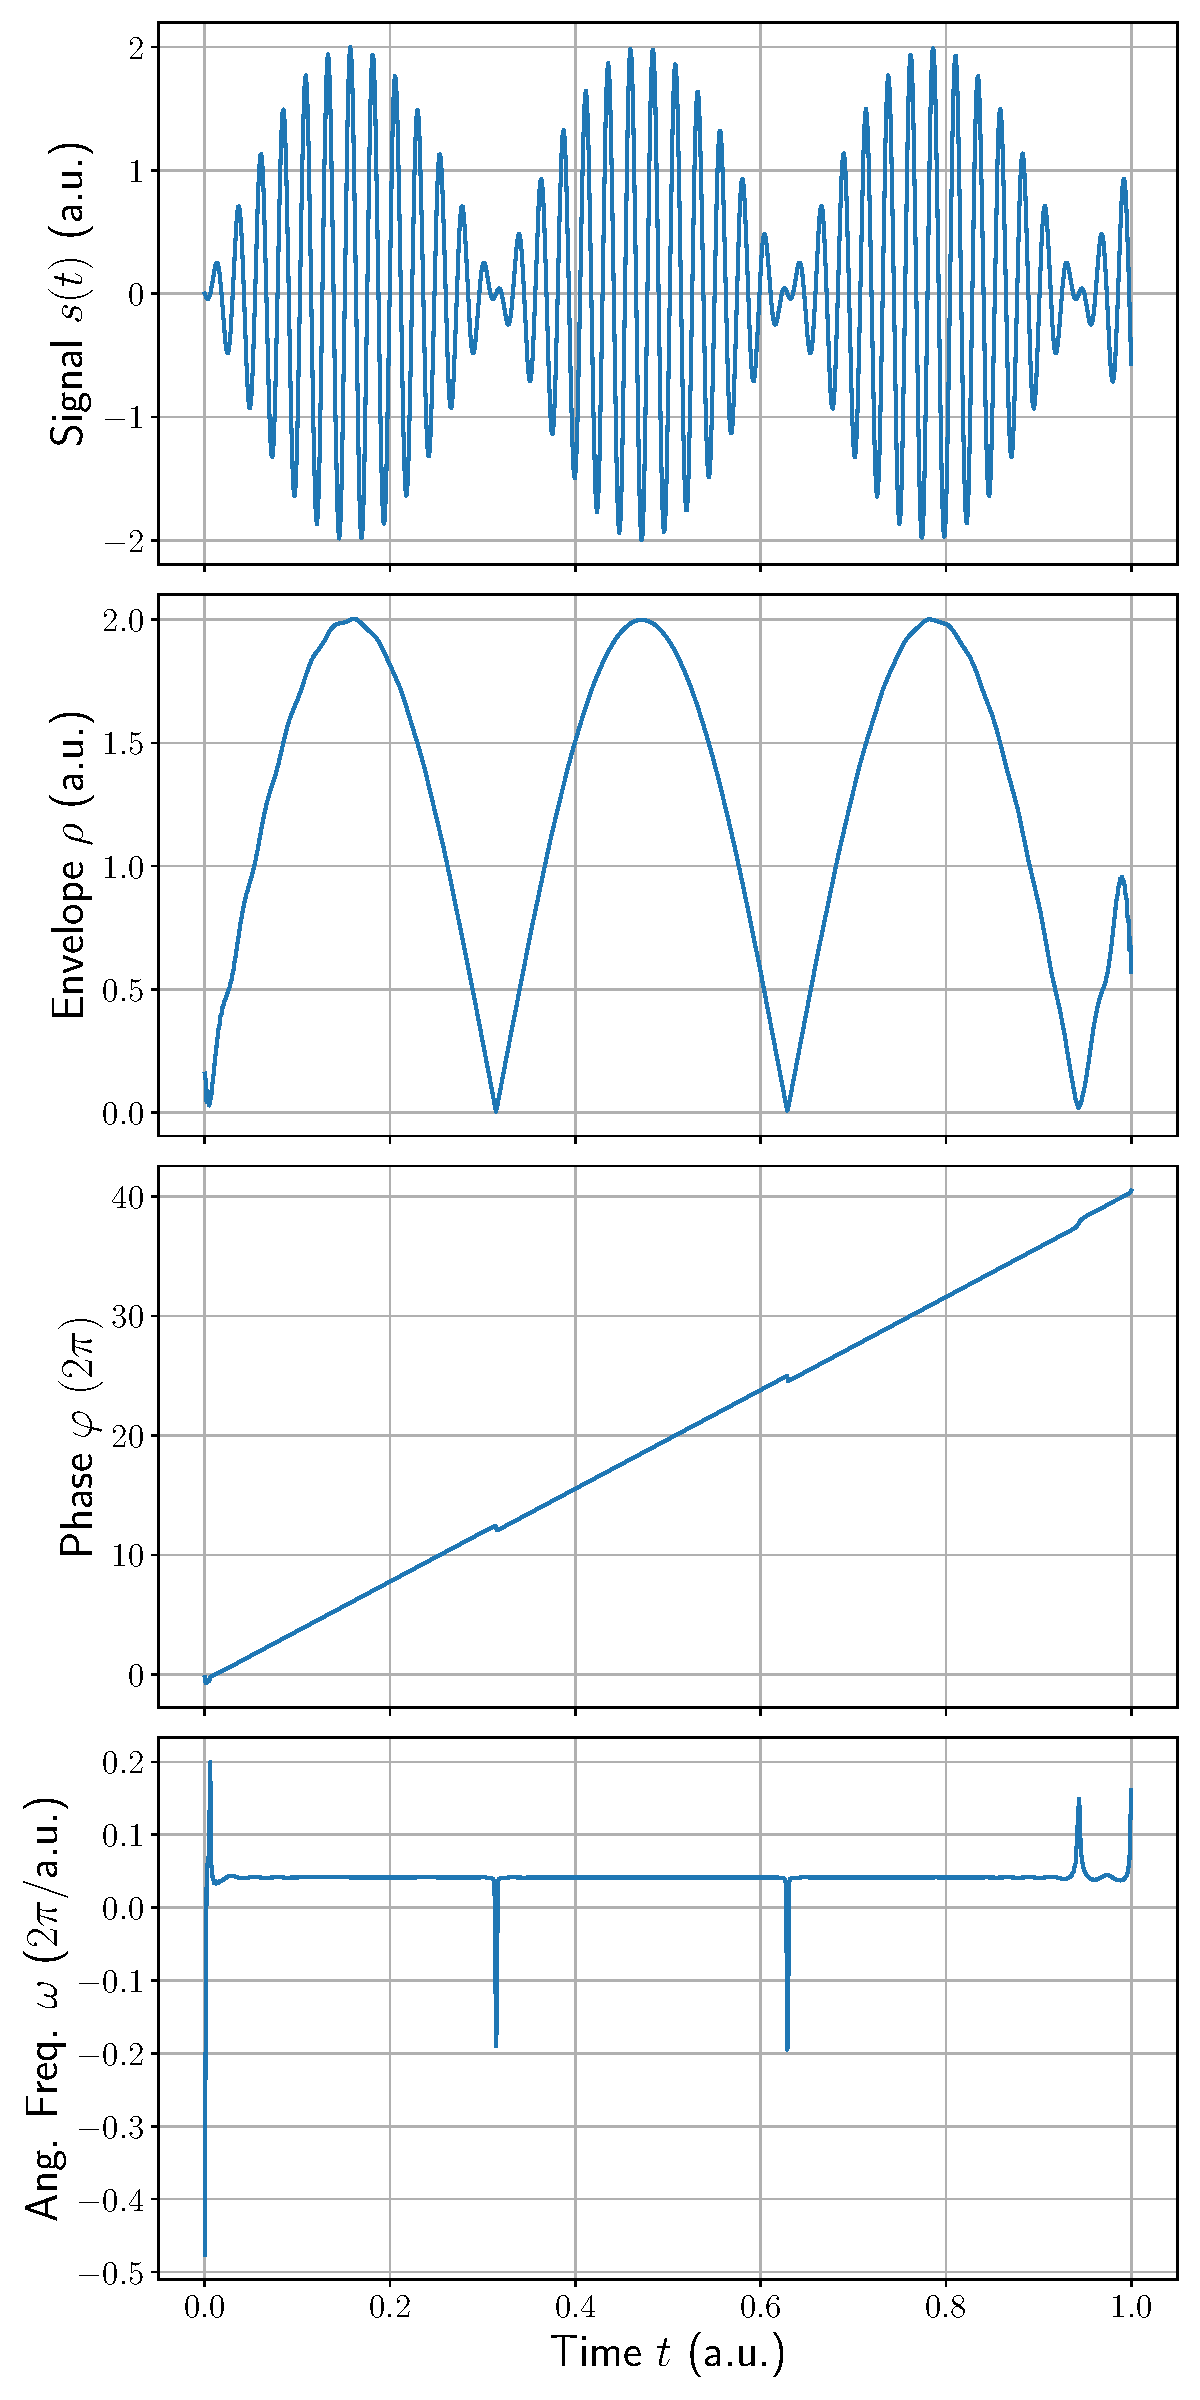
\includegraphics[width=0.6\textwidth]{../analytic_sig.pdf}
    \caption{Provided signal and its envelope, phase and angular frequency obtained via the method of the analytical signal.}
    \label{fig:ts}
\end{figure}
We apply the method of the analytical signal to the provided time series using the \texttt{hilbert} function from the \texttt{scipy} package. Note that we correct for phase jumps when $\phi$ reaches the bounds of $[0, 2\pi]$ using the \texttt{unwrap} function from \texttt{numpy}. The results are shown in figure~\ref{fig:ts}. We can see that except for some small phase jumps which are likely numerical artefacts, the phase increases linearly with time corresponding to a monochromatic angular frequency. The envelope has a frequency of its own which we do not determine explicitly.
\subsection{}
\begin{figure}
    \centering
    \begin{subfigure}{0.49\textwidth}
        \centering
        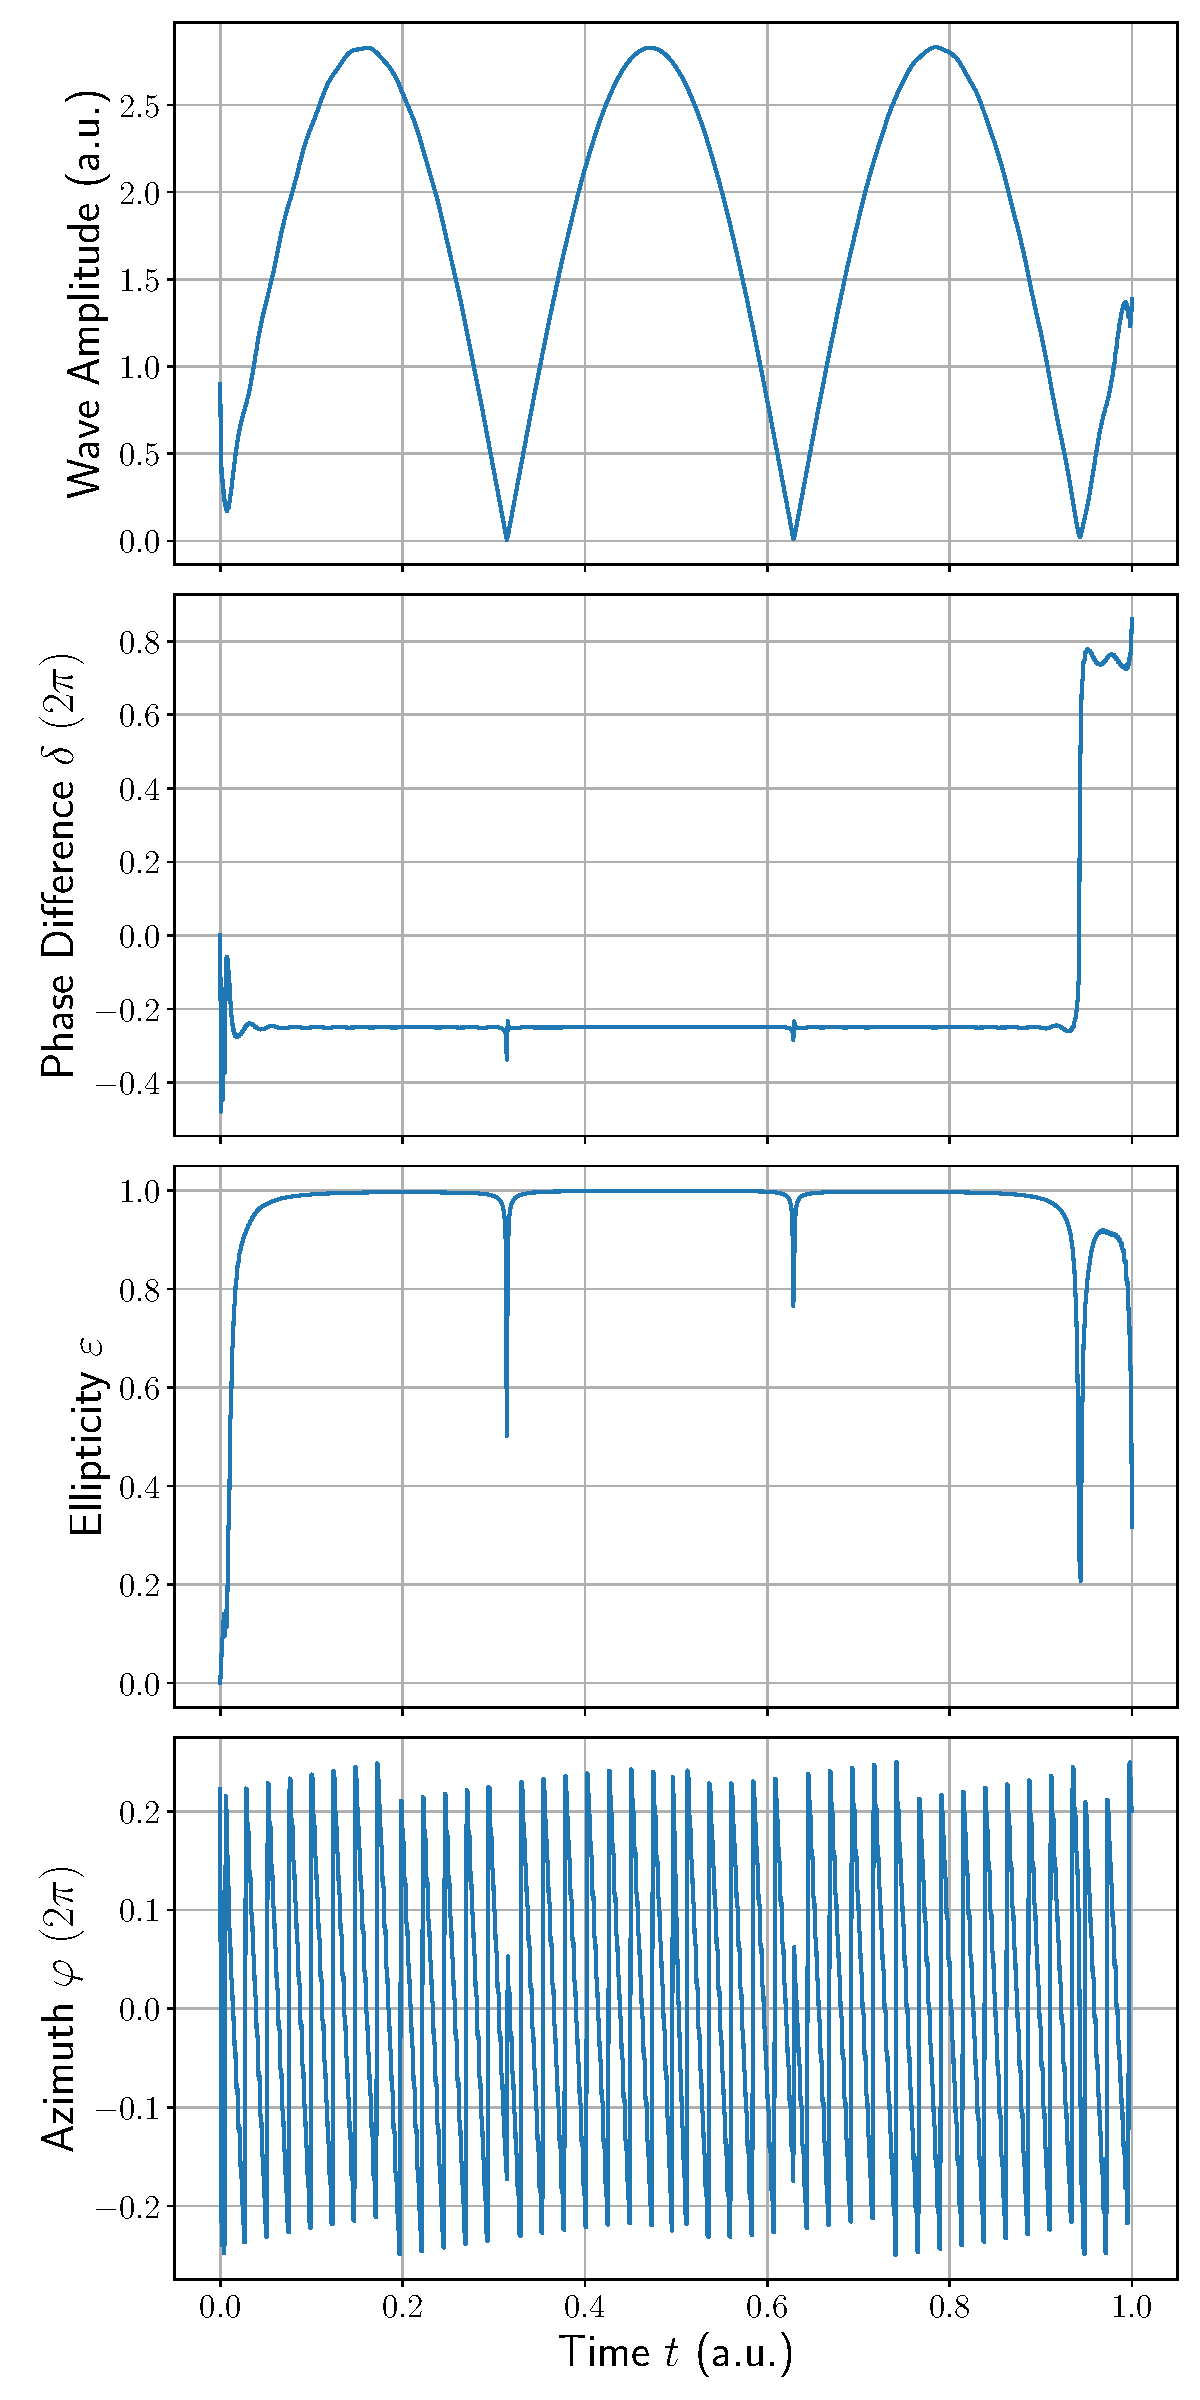
\includegraphics[width=\textwidth]{../wave1.pdf}
        \caption{Wave 1}
        \label{subfig:wave1}
    \end{subfigure}    
    \begin{subfigure}{0.49\textwidth}
        \centering
        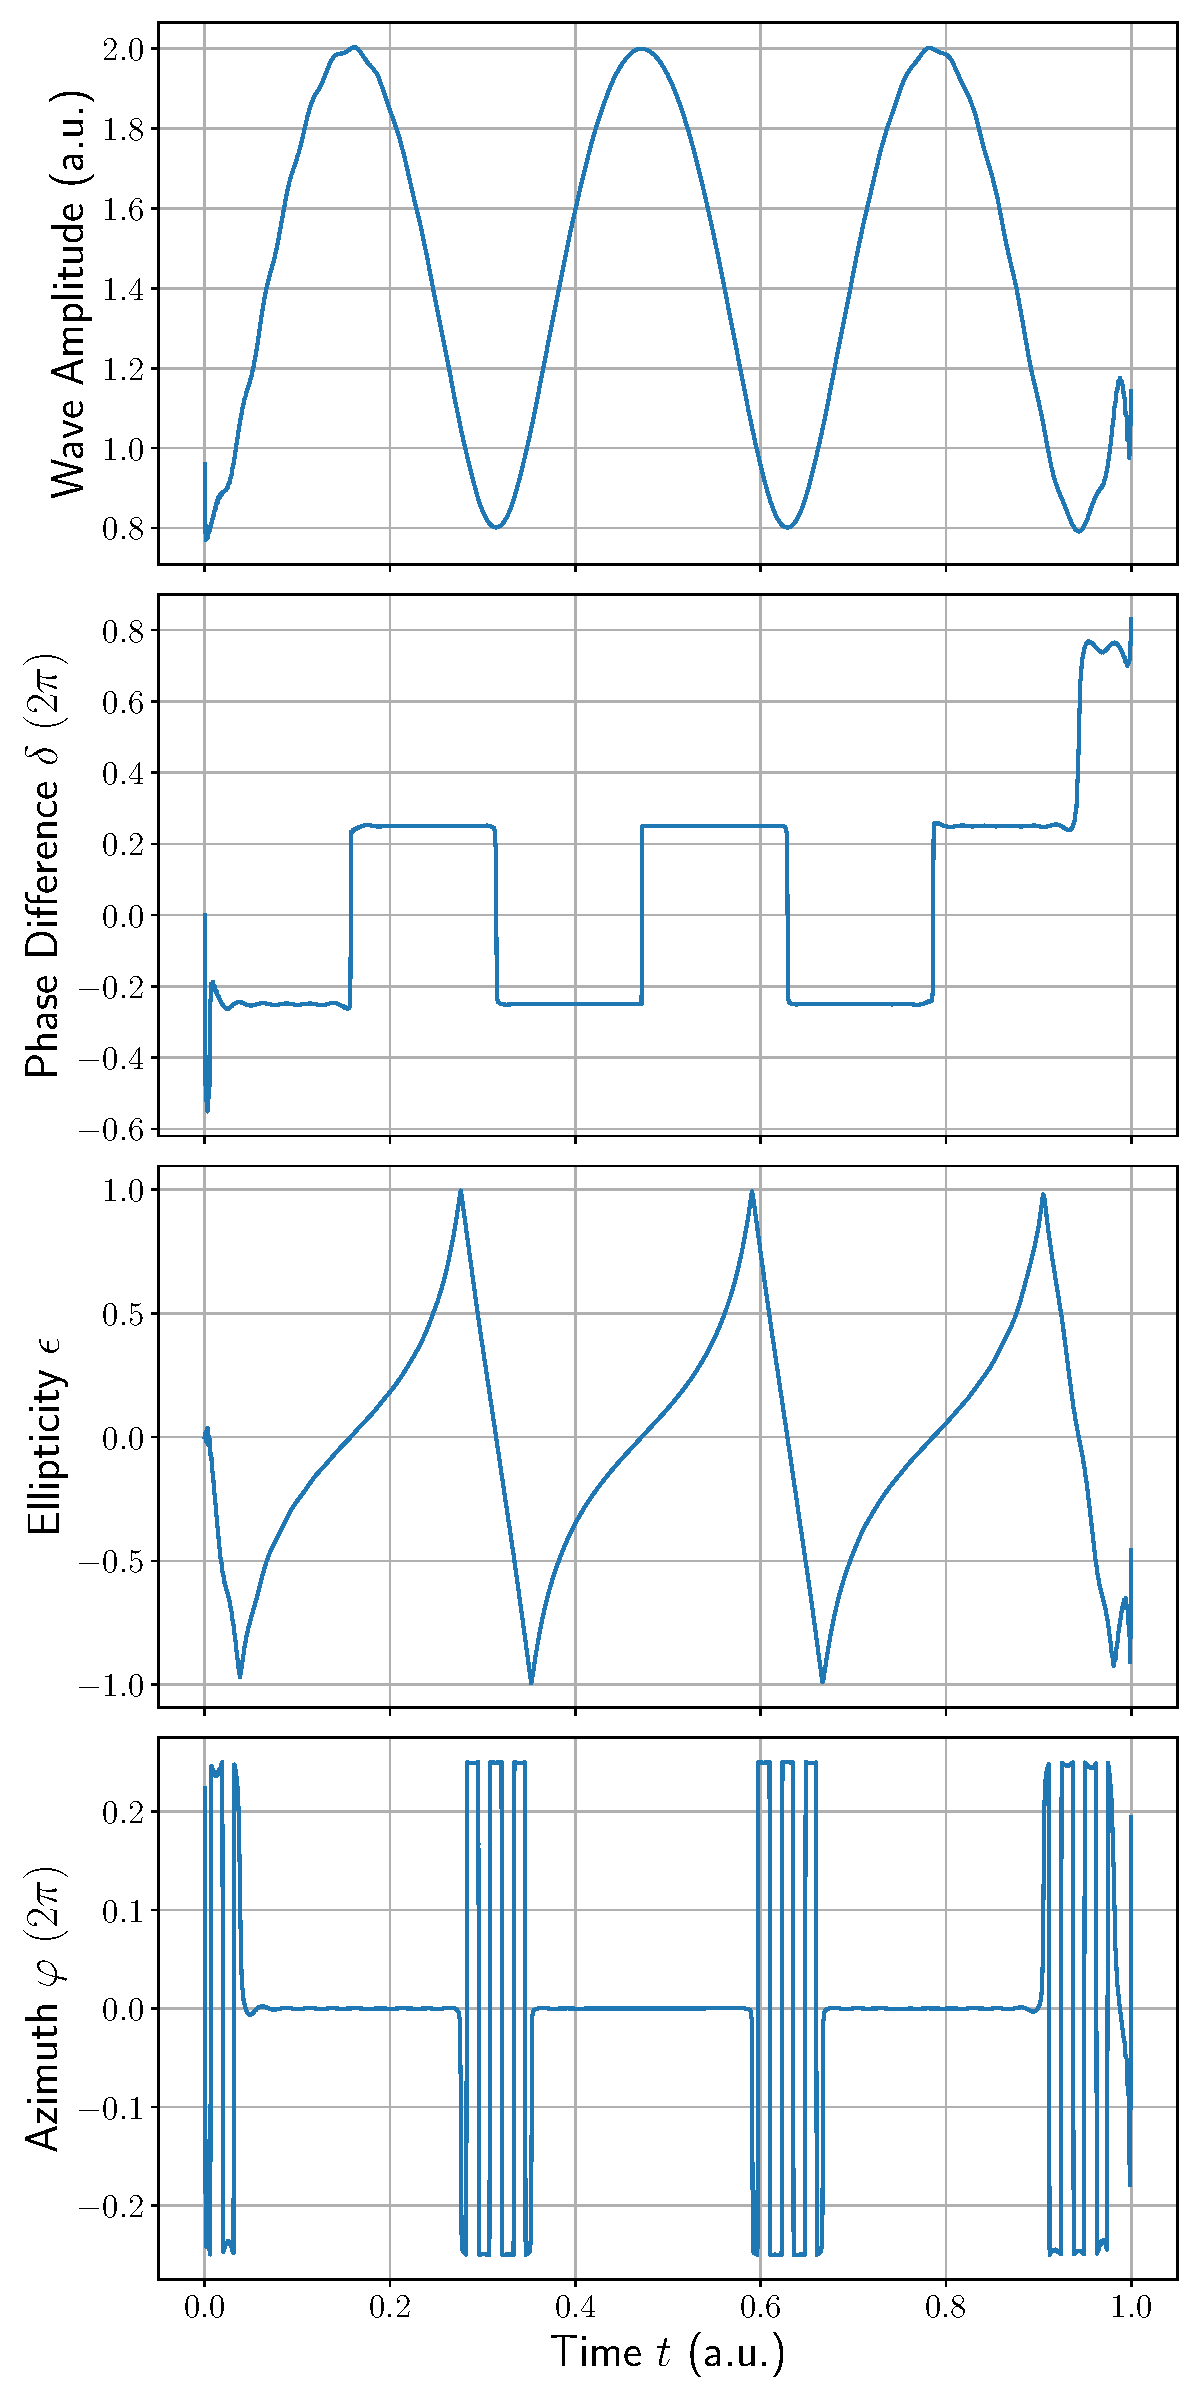
\includegraphics[width=\textwidth]{../wave2.pdf}
        \caption{Wave 2}
        \label{subfig:wave2}
    \end{subfigure}    
    \caption{Amplitude, phase difference $\delta$, ellipticity $\varepsilon$ and azimuth $\varphi$ of the two given waves.}
    \label{fig:waves}
\end{figure}
We employ equations (115) through (119) in the lecture notes to determine the phase difference $\delta$, ellipticity $\varepsilon$ and azimuth $\varphi$ of the two waves, however we plot the absolute value of $\varepsilon$ as it is given in the scriptum because it is to be interpreted as the ratio of the two semi-axes of the instantaneous ellipse of the signal which should not assume negative values. The results can be seen in figure~\ref{fig:waves}. 

We can see that wave one is almost perfectly circular over a large range of the signal, with deviations toward the end which can also be seen in the other quantities. For a circular signal, the azimuth is meaningless. The phase difference remains constant up until the end of the signal where there is a jump in phase of absolute value $2\pi$, which is not meaningful.

For the second wave, there are repeated phase jumps back and forth of absolute value $\pi$. The ellipticity is also constantly varying, but its extrema do not coincide with the jumps in phase. The ellipticity going to zero seems to indicate that one of the components of the wave goes to zero periodically. When this happens, the azimuth jumps by $\pi$.
\FloatBarrier
\newpage
\section{Nyquist Frequency}
\begin{figure}[h]
    \centering
    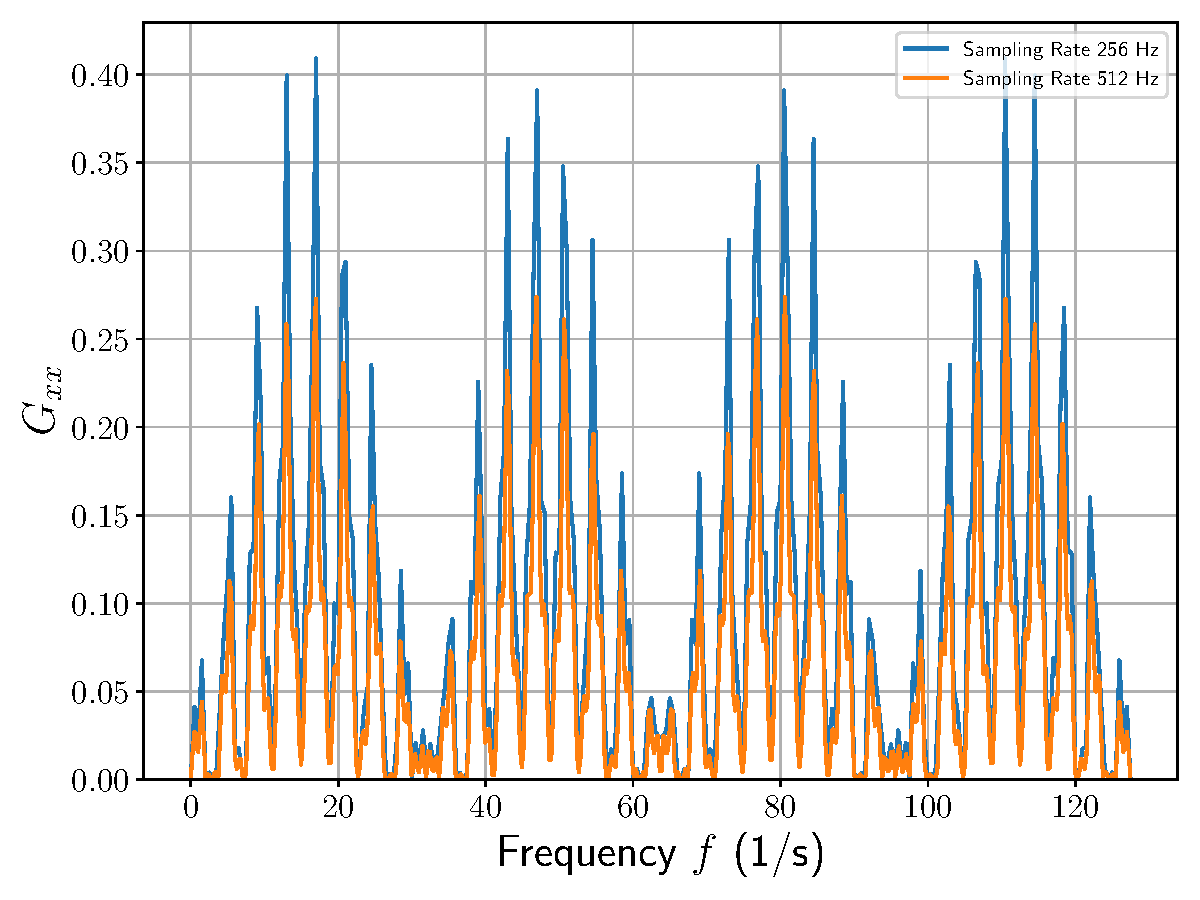
\includegraphics[width=0.7\textwidth]{../G.pdf}
    \caption{Discrete one-sided auto-spectral density $G_{xx}$ of the provided function using different sampling frequencies.}
    \label{fig:g}
\end{figure}
Figure~\ref{fig:g} shows the one-sided auto-spectral density of the given function $y(t)$ for different sampling rates. Given the fact that the highest frequency present in the function is 128 Hz, it is immediately clear from the sampling theorem that we will have to use a sampling frequency of at least 256 Hz to correctly represent the spectrum of $y$. This can be seen in the figure, where for 50 Hz, not even the 32 Hz component can be resolved. Only at 256 Hz are all peaks in the spectrum where they should be. The height of the peaks corresponds to the amplitude of the respective component.

\FloatBarrier
\newpage
\section{Correlation Function and Fourier Transformation}
\subsection{}
\begin{figure}[h]
    \centering
    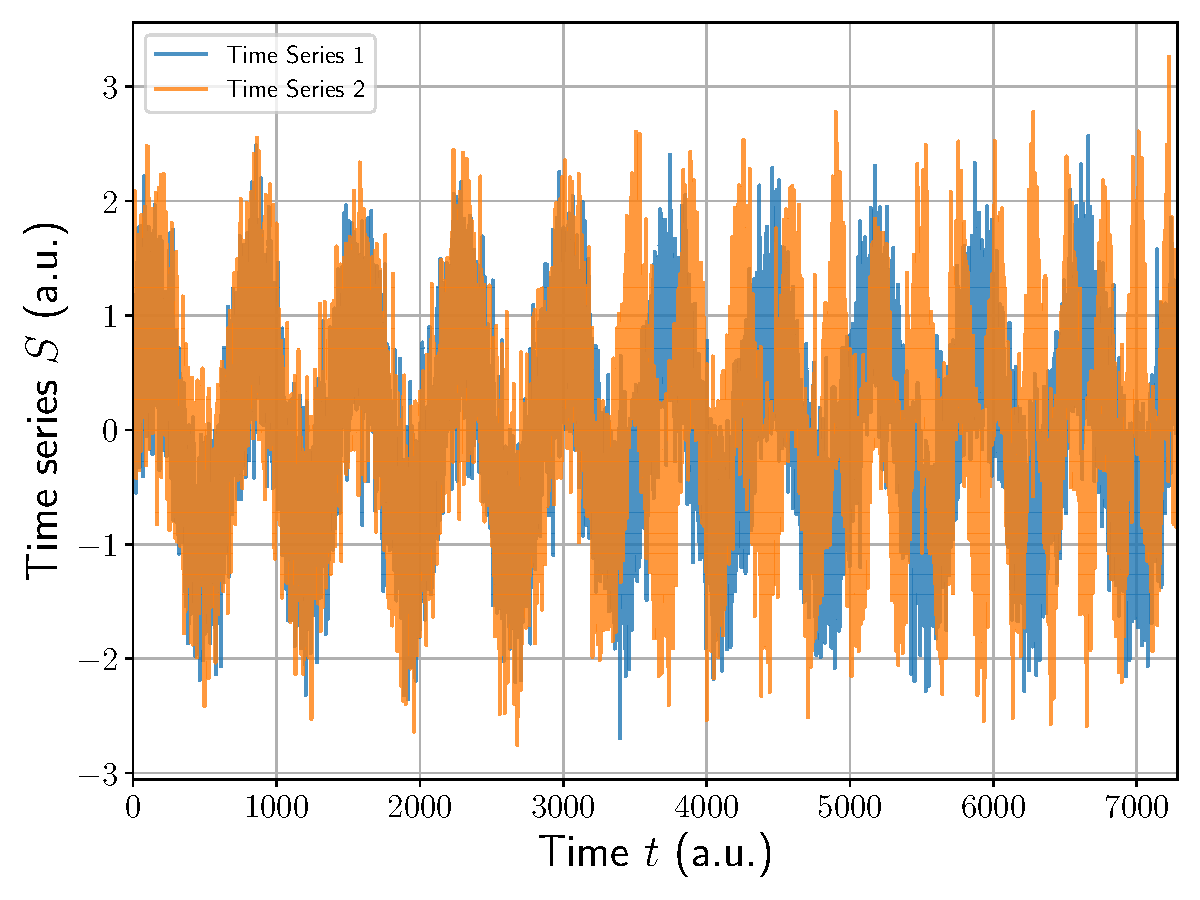
\includegraphics[width=0.6\textwidth]{../ts.pdf}
    \caption{Time series 1 and 2 as provided.}
    \label{fig:ts3}
\end{figure}
Figure~\ref{fig:ts3} shows the two time series. We can see that their low-frequency behaviour is initially congruent but the frequency of time series 2 ramps up towards larger times compares to time series 1.
\subsection{}
\begin{figure}
    \centering
    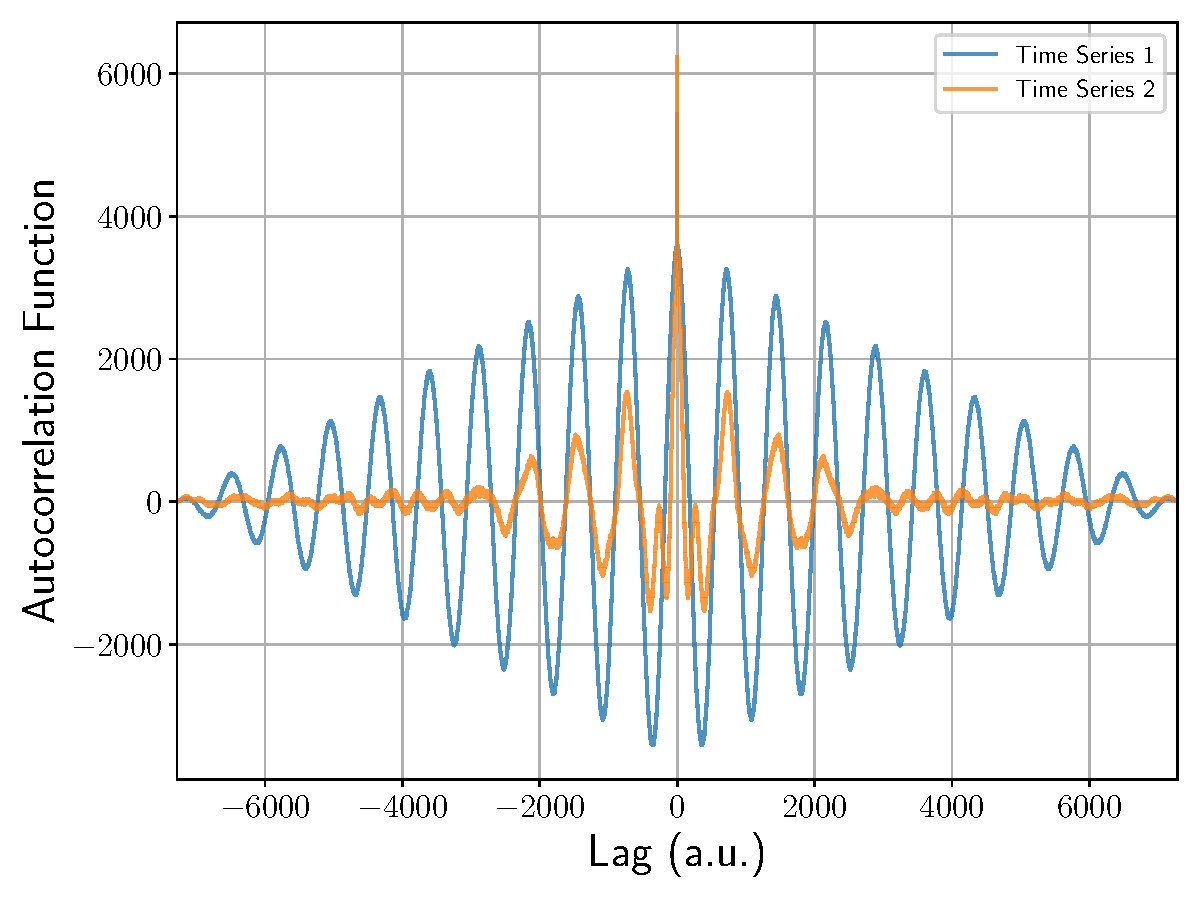
\includegraphics[width=0.6\textwidth]{../ac.pdf}
    \caption{Auto-correlation function of time series 1 and 2.}
    \label{fig:ac}
\end{figure}
The auto-correlation functions of both time series are shown in figure~\ref{fig:ac}. Both exhibit the expected spike at zero lag. Time series one's constant period exhibits itself in the periodic peaks of the auto-correlation. The fall-off in the height of these peaks can be understood as a numerical artefact due to the finite sample of the signal. Time series two's peaks are not equidistant owing to its changing frequency.
\subsection{}
\begin{figure}
    \centering
    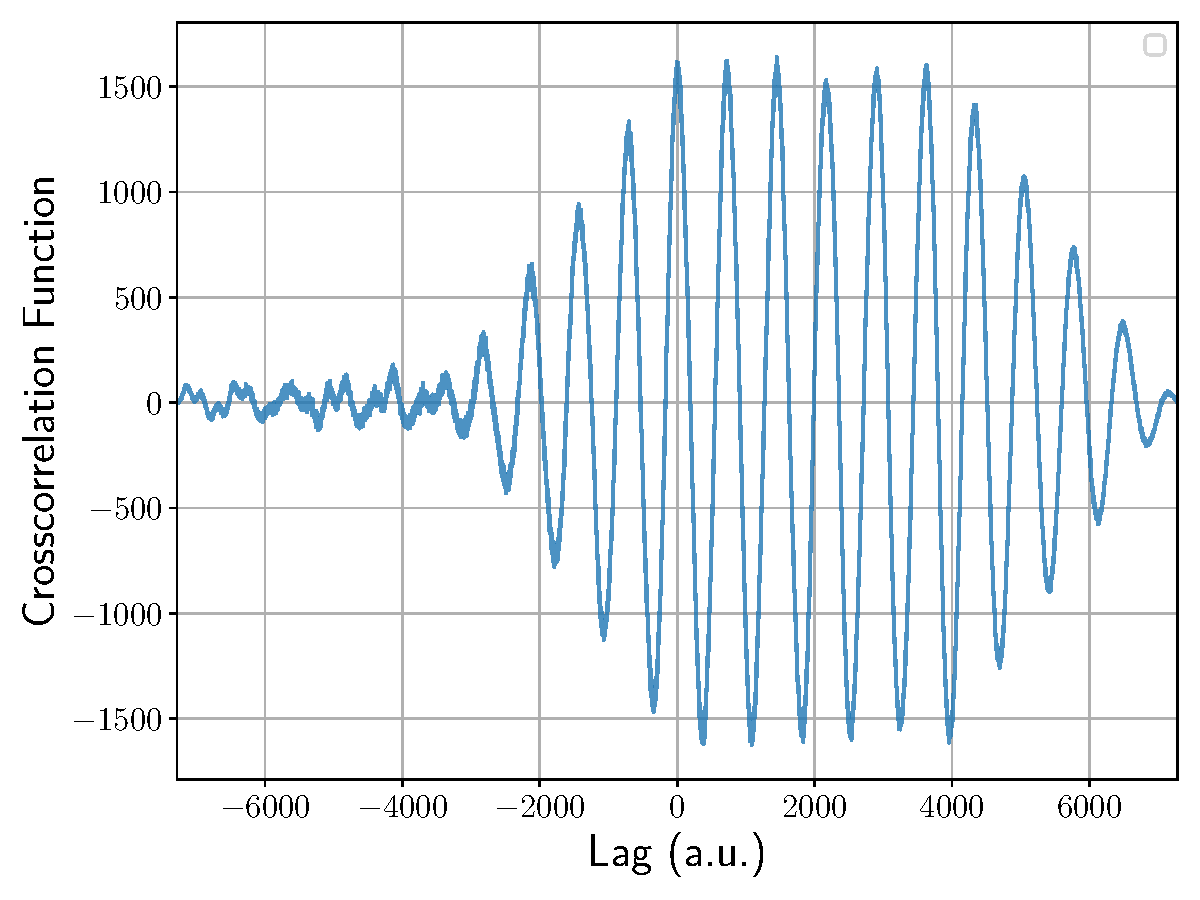
\includegraphics[width=0.6\textwidth]{../cc.pdf}
    \caption{Cross-correlation function of time series 1 and 2.}
    \label{fig:cc}
\end{figure}
The cross-correlation function of both time series is shown in figure~\ref{fig:cc}. Other than the auto-correlation functions, it is not symmetrical about the lag. This is because of the changing frequency of signal two and the finite sample and the associated zero-padding used by \texttt{scipy}. When we move the beginning of time series 2 onto the end of time series two, the absolute value of the correlation is large (subject to aligning the peaks with peaks or troughs) because the frequencies match, but if we shift the beginning of signal 1 onto the end of signal two, they no longer do. 
\subsection{}
\begin{figure}
    \centering
    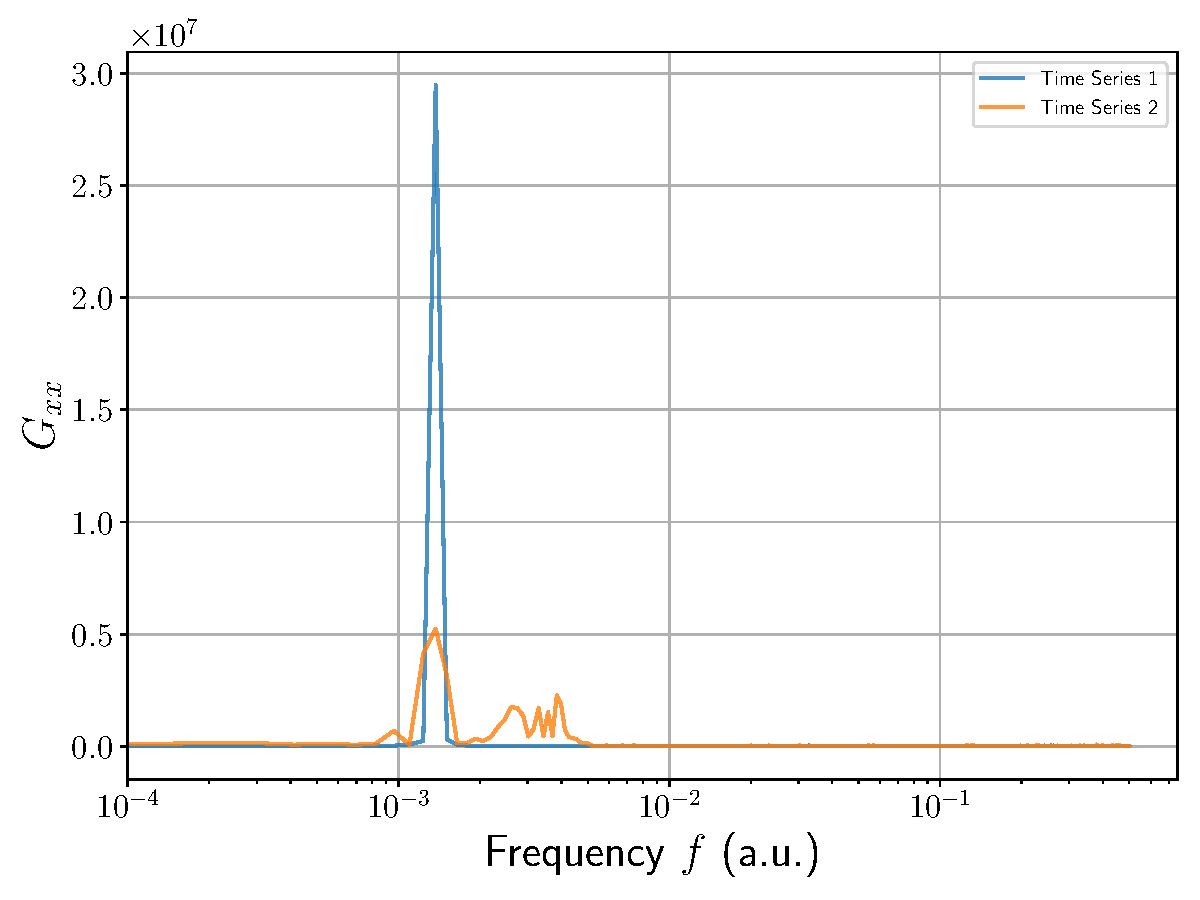
\includegraphics[width=0.6\textwidth]{../G_03.pdf}
    \caption{One-sides auto-spectral density of time series 1 and 2.}
    \label{fig:g_3}
\end{figure}
Figure~\ref{fig:g_3} shows the spectral densities of both signals. We can see that time series 1 has a sharp peak due to its monochromatic nature whereas time series two also shows a peak at that frequency but also peaks at higher frequencies as expected.
\subsection{}
At this point we got lazy.

\end{document}